\documentclass{subfiles}

\begin{document}



\section{The Importance of Dead Wood}

\par The value of dead trees from a biodiversity management perspective is large. Once a tree dies, its contribution to our ecosystem continues. The woody structure remains for centuries and it contributes to forest regeneration while providing resources for numerous surrounding organisms \cite{Franklin1987}. As an indication, more than 4000 species inhabit dead wood in Finland \cite{Siitonen2001}, where an estimate of 1000 species has been extinct \cite{Hanski2000}. These species do not only include animals and birds but also organisms, like fungi. Fungi contributes to wood decaying, formation of hollows and biodiversity, which is an important factor for a resilient ecosystem \cite{Peterson2000}. Observing the changes of fungal diversity on decaying wood has an increased interest in science  \cite{Abrego2011} \cite{Stokland2011} \cite{Lonsdale2008} in order to ensure the continuous existence of decaying wood in forests. 




\par Specifically in Australia, tree hollows play a significant role in managing biodiversity. Nearly all arboreal mammals rely on hollows with the exception of the Koala and perhaps Ringtail Possums that preferentially make a stick nest, but they use hollows as well. Additionally, a large number of Australian bird species rely on hollows for shelters \cite{Gibbons2002}. Nevertheless, Australia has no real hollow creators like the northern hemisphere (e.g. Woodpeckers), and therefore it relies predominantly on natural processes of limb breakage, insect and fungal attack when access points are provided through damage caused by wind, storms and fire. These kind of hollows take hundreds of years to form and because of that it is more likely to exist on dead trees. In Australia, studies predict shortage of hollows for colonisation in the near future \cite{Lindenmayer2010} \cite{Goldingay2009}, therefore automated detection of them plays a significant role in protecting those animals. As an indicator of the importance of hollows in managing biodiversity, a few species that rely on hollows was provided as list by the Forestry Corporation of NSW. Those species are shown at Figure \ref{fig:Birds}. According to the Department of the Environment of Australian Government and the Government of Western Australia sixe of them are  protected, threatened or close to extinct \cite{AustraliaExtinct1999}  \cite{AustraliaExtince2015}. In Figure \ref{fig:Birds}, those six species have a red border and their names are bold in its description. 

\par For the aforementioned reasons, monitoring dead trees is essential for having a resilient ecosystem. Nevertheless, the distribution of dead trees significantly varies making detection of them difficult \cite{Kim2009}. Remote sensing approaches has been introduce to automate the process of monitoring forest and further increase the spatial resolution of the monitored area. The following section gives an overview of the related work undertaken in Remote Sensing. 



\afterpage{
    \begin{figure} 
    	\centering
    	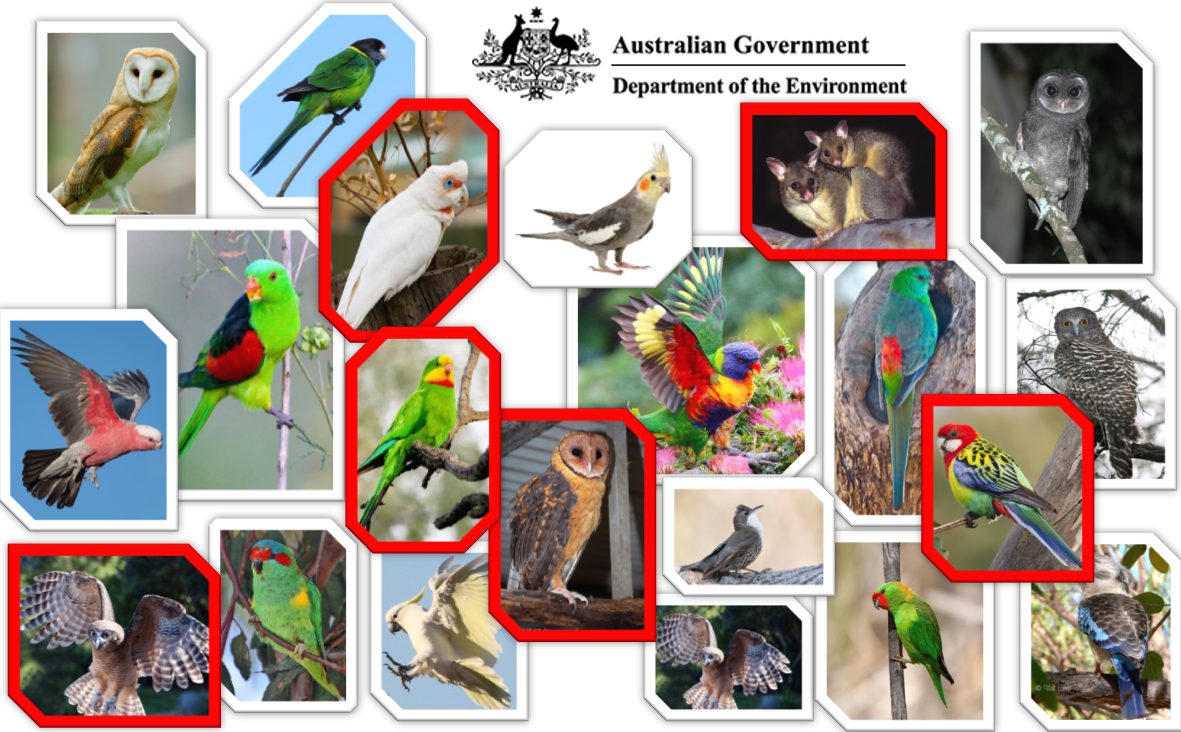
\includegraphics[width=\textwidth]{img/Birds}
    	\caption[Animals Closes to Exctinction]{A number of species that rely on tree hollows of which the red ones / bold ones are close to extinction: Kookaburra, Sulphur Crested Cockatoo, \textbf{Corella},  Crimson Rosella, Eastern Rosella,  Galah, Rainbow Lorikeet,  Musk Lorikeet, Little Lorikeet , Red-winged Parrot,  \textbf{Superb Parrot}, Cockatiel,   Australian Ringneck (Parrot),  Red-rumped Parrot,   Powerful Owl,    Sooty Ow,        Barking Owl, \textbf{Masked Owl},  \textbf{Barn Owl},  White-throated Treecreeper, Hollow Owl, \textbf{Brush-tailed Possum} (mammal) \footnotemark}
    	\label{fig:Birds}
    \end{figure}
    \footnotetext{    	
        The images of the birds were taken from the following links (Retrieved on the 27th of April 2016):  
    	Kookaburra: \url{<http://tenrandomfacts.com/blue-winged-kookaburra/>}, 
    	Sulphur Crested Cockatoo: \url{<http://aussiegal7.deviantart.com/art/Sulphur-Crested-Cockatoo-08-153341893>},
    	Corella: \url{<http://www.theparrotplace.co.nz/all-about-parrots/long-billed-corella/},     	Superb Parrot: \url{<http://www.davidkphotography.com/?showimage=637>},
    	Crimson Rosella: \url{<http://25.media.tumblr.com/tumblr_m3mo89c40r1r4t9h1o1_1280.jpg>},
    	Eastern Rosella: \url{<http://2.bp.blogspot.com/-pYxw51WjSOY/UB-LEFgd2KI/AAAAAAAAAWg/9z60PUWE6TE/s1600/_GJS6601-as-Smart-Object-1.jpg>},
    	Rainbow Lorikeet: \url{<https://www.reddit.com/r/pics/comments/328fvc/a_rainbow_lorikeet_found_in_coastal_regions/>},     	Musk Lorikeet: \url{<http://www.rymich.com/girraween/photos/animals/birds/medium/glossopsitta_concinna/glossopsitta_concinna_001.jpg>},     	Little Lorikeet: \url{<http://www.pbase.com/sjmurray/psittacidae>},     	Red-winged Parrot: \url{<https://www.pinterest.com/pin/395894623469889727/>}, Cockatiel: \url{<http://up.parsipet.ir/uploads/Cockatiels-for-sale.jpg>},     	Australian Ringneck (Parrot): \url{<http://ontheroadmagazine.com.au/wp-content/uploads/2015/09/Twenty-eight-parrot-2-min.jpg>},     	Red-rumped Parrot: \url{<http://parrotfacts.net/wp-content/uploads/Red-Rumped-Parrot-on-a-tree.jpg>},     	Powerful Owl: \url{<http://farm1.staticflickr.com/219/495796536_f78dac04c1.jpg>},     	Sooty Owl: \url{<ttp://www.mariewinn.com/marieblog/uploaded_images/screech2-738532.jpg},     	Barking Owl: \url{<http://www.pcpimages.com/Nature-and-Wildlife/Birds/i-7JKSTp5/1/L/owl\%20\%281\%20of\%201\%29-L.jpg>},     	Masked Owl: \url{<http://www.survival.org.au/images/birds/masked_owl_2_600.jpg>},  	Galah: \url{https://www.pinterest.com/pin/537546905498955709/>},   	White-throated Treecreeper: \url{<https://geoffpark.files.wordpress.com/2011/09/female-white-throated-treecreeper.jpg>}, Hollow Owl: \url{<http://www.mariewinn.com/marieblog/uploaded_images/screech2-738532.jpg>} }
}





\section{Related Work}

\par Remote Sensing was introduced in monitoring dead trees in forests in order to improve detection due to their variance spread. Dead trees could either be fallen or standing. The task of identifying those types of them is different from a classification perspective. Fallen trees are identified by detecting segments or line-like features on the terrain surface using LiDAR data \cite{Polewski2015} \cite{Mucke2013}. Regarding standing dead trees, their shape (reduced number of leaves or broken branches) \cite{Yao2012} and light reflectance (less green light illuminated) \cite{Pasher2009} are important factors for identifying them.


\par Previous work on dead standing trees detection, suggests single tree segmentation before dead trees identification \cite{Yao2012}.
Research on top tree detection with maxima and watershed for delineation. 



 \par This research is focused on standing dead tree detection and to be more specific in native Eucalypt forest in Australia. In case of Eucalyptus single tree detection is a challenge on its own due to their irregular structure and multiple trunk splits. 

Tree delineation from bottom to top \cite{Shendryk2016_treeDeliniation} 



An interesting work for delineating Eucalyptus recommends delineation from bottom to top. It first identifies standing trunks and then segments the points cloud. 

This is then used for monitoring forest health \cite{Shendryk2016_DeadTrees}



Nevertheless, this approach is time consuming and here it is introduced a fast approach for rough classification similar to boost cascade \cite{Viola2001} but extended to 3D. 

Dong, 2009, introduced 3D tree shape signatures for distinguishing Oaks from Douglas fir tree crowns. The 3D shape signatures were generated by getting the distance distribution of random LiDAR point pairs of the two tree crown classes: Oaks and Douglas \cite{Dong2009}. 

	\begin{figure} [h!]
		\centering
		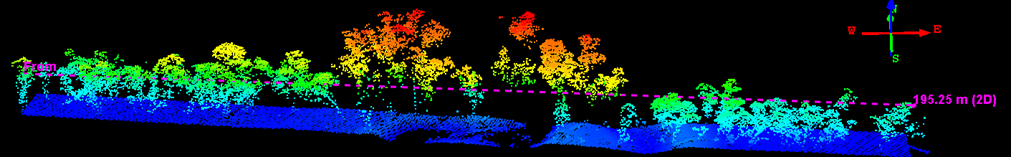
\includegraphics[width=\textwidth]{img/TreesNoTrunks}
		\caption{LiDAR point cloud showing that there are very limited points reflected from tree trunks.}
		\label{fig:NoTrunks}
	\end{figure}


\par Traditional ways of interpreting FW LiDAR data, suggests extraction of a denser points cloud using Gaussian decomposition ~\cite{Neuenschwander2009} ~\cite{Reitberger2008}. Nevertheless DASOS was influenced by Persson et al, 2005, who used voxelisation to visualise the waveforms ~\cite{Persson2005}. But, DASOS do not only uses voxelisation for visualisations but also for extracting metrics useful in classification. It further normalises the intensities so that equal pulse length exists inside each voxel, making intensities more meaningful. It is further seems that the literature is moving towards voxelisation with the good results obtained at recent publication on tree species classification ~\cite{Cao2016}. 

\section{Data and Fieldplots}

\par The data, provided by RPS Australia East Pty Ltd, were collected in March 2015 from the Riegl ( LMS-Q780 or LMS-Q680i?) sensor at an Australian native Forest with eucalyptus. The fieldplots has been provided by (Interprine Group Ltd or Forest Corporation?). 
The LiDAR data used for this project are provided by RPS Australia East Pty Ltd and they were collected in March 2015 using the Riegl ( LMS-Q780 or LMS-Q680i?) sensor. The Riegl LMS-Q??? is a native full-waveform sensor and the LiDAR point clouds were generated from the waveform instrument data during post processing. In addition, the field plots used for the classifications are provided by (Interprine Group Ltd or Forest Corporation?) and contain around 1000 Eucalypt trees while 10\verb|%| of them are dead. 

33 plots allocated randomly in the area of interest
Plot Radius: 35.68m 
GPS tree location
Tree information like Dead trees
2386 Trees 
269 Dead Trees


\section{Actual Data and Problem}

\begin{figure} [h!]
	\centering
	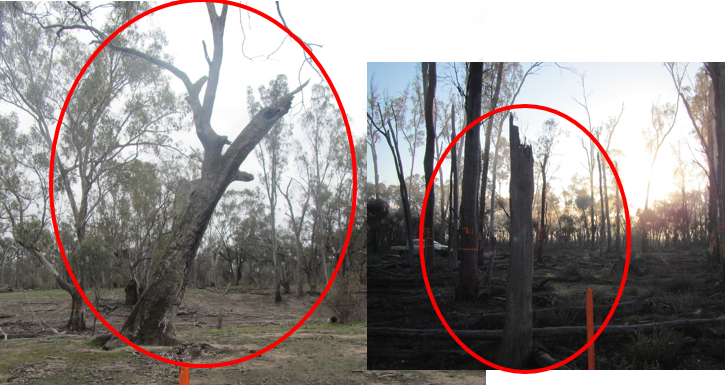
\includegraphics[width=\textwidth]{img/DeadTreesExamplePhotos}
	\caption{The shape of dead trees significantly varies from the each other. Here there is an example of two dead trees.}
	\label{fig:DeadTreesExamplePhotos}
\end{figure}


	\begin{figure} [h!]
		\centering
		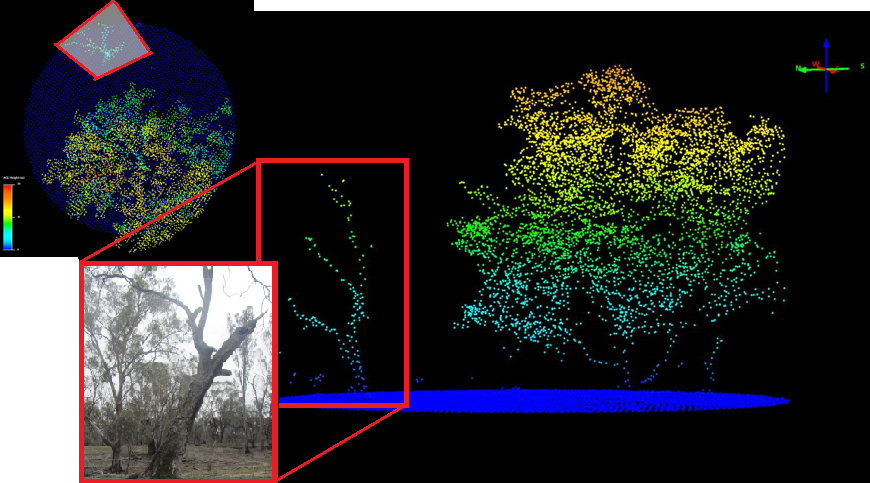
\includegraphics[width=\textwidth]{img/DeadTreeInLiDAR}
		\caption{Example of a dead tree in relation to the discrete LiDAR point cloud.}
		\label{fig:DeadTreeInLiDAR}
		\end{figure}
		
		
		

\section{Methodology}

\par In this chapter, the 3rd feature of DASOS (Table \ref{tbl:functionalities}) is used for generating 3D priors characterising dead standing Eucalypt trees. These 3D priors are used for detecting dead standing Eucalypt trees in native Australian forests. 

\section{Experiments and Results}

\section{Conclusions}













\end{document}